% Tikz File 'IC_temp.tex'
\documentclass{standalone}
\usepackage{tikz}
\usetikzlibrary {arrows.meta} 
\begin{document}
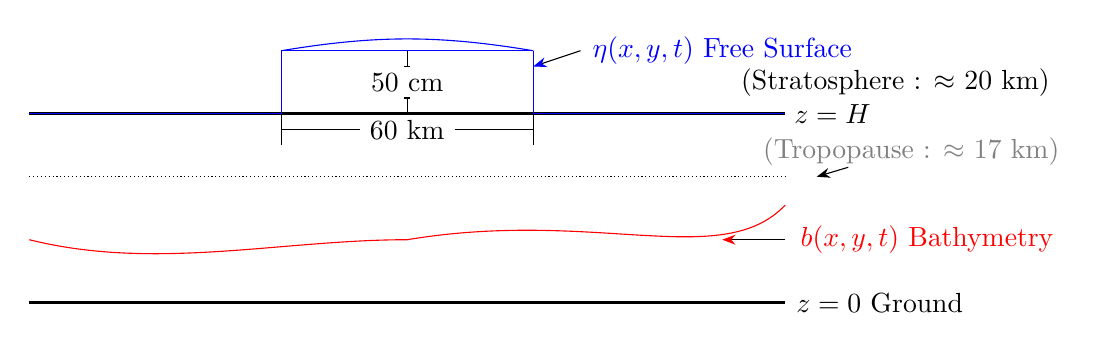
\begin{tikzpicture}[scale=0.4]
		\draw[very thick] (-12,0) -- (12,0);
		\draw[very thick] (-12,6) -- (12,6);
		\draw[blue] (-12,6) -- (-4,6);
		\draw[blue] (-4,6) -- (-4,8);
            \draw[blue] (4,6) -- (4,8);
            \draw[blue] (-4,8) -- (4,8);
		\draw[blue] (4,6) -- (12,6);
  		\draw[red] (-12,2) .. controls (-8,1) and (-4,2) .. (0,2);
		\draw[red] (0,2) .. controls (6,3) and (10,1) .. (12,3.1);
		\node at (13.5,6) {$z=H$};
            \node at (15.5,7) {(Stratosphere : $\approx$ 20 $\mathrm{km}$)};
		\node at (15,0) {$z=0$ Ground};
		\draw[-{Stealth[blue]}] (5.5,8)   -- (4,7.5);
		\node[blue] at (10,8) {$\eta(x,y,t)$ Free Surface};
		\draw[-{Stealth[red]}] (12,2.0)   -- (10,2);
		\node[red] at (16.5,2) {$b(x,y,t)$ Bathymetry};
            \draw[blue] (-4,8) .. controls (-1,8.5) and (1,8.5) .. (4,8);
		\draw(0,6) -- (0,6.5);
		\draw(-0.1,6.5) -- (0.1,6.5);
		\draw(0,8) -- (0,7.5);
		\draw(-0.1,7.5) -- (0.1,7.5);
		\node at (0,7) {50 cm};
            \draw(-4,6) -- (-4,5);
            \draw(4,6) -- (4,5);
            \draw(-4,5.5) -- (-1.5,5.5);
            \draw(1.5,5.5) -- (4,5.5);
            \node at (0,5.5) {60 km};
  \draw[densely dotted ] (-12,4) -- (12,4);
  \draw[-{Stealth[black]}] (14,4.3)   -- (13,4);
  \node[gray] at (16,4.8) {(Tropopause : $\approx$ 17 $\mathrm{km}$)};
	\end{tikzpicture}
\end{document}